\section{Part 2: SSVEP Analysis}

\begin{taskbox}[Part 2: introduction in the lab manual]
The file \texttt{SSVEP\_EEG.mat} contains the SSVEP signal recorded from one user. This file contains a matrix \texttt{SSVEP\_Signal} (EEG recorded from 6 channels Pz, Oz, P7, P8, O1 and O2, with sampling frequency 250 Hz), a matrix \texttt{Events} (stimulation frequencies) and a matrix \texttt{Event\_Samples} (the time sample corresponding to the start of each stimulus). The goal is to determine the stimulation frequency from the EEG signal recorded in each trial.
\end{taskbox}

\subsection*{(a) Data and band-pass filter}
\begin{taskbox}
For each channel of the data, use a band-pass filter to remove the frequencies below 1 Hz and above 40 Hz. For each channel, plot the denoised signal together with the original signal in one graph.
\end{taskbox}

The SSVEP signal consists of six channels, Pz, Oz, P7, P8, O1 and O2, sampled at 250~Hz. For 15 stimuli, the goal is to detect the fundamental stimulation frequency from the EEG and to examine the differences between the responses of the channels. Five frequencies, 6.5, 7.35, 8.3, 9.6 and 11.61~Hz, were each recorded three times. According to the basis of the lab notes, the SSVEP response can have components at the stimulation frequency and at its integer multiples.

For each of the six channels, a Butterworth band-pass filter with cutoffs of 1 and 40~Hz, implemented with second-order sections, was designed. The order of the initial prototype is four, and the final band-pass order is eight in each pass. The filter was applied forward and backward on the continuous signal so as not to create phase delay in the offline analysis; in this case the amplitude response equals the square of the amplitude response of the single pass. Filtering before cutting the repetitions prevents a separate transient at the beginning of each repetition.

The comparison of the raw and the filtered recording shows the removal of most of the slow trend and of the out-of-band variations. A real filter has a gradual transition; cutoffs of 1 and 40~Hz do not mean an ideal, sudden removal of all power outside this range.

\begin{figure}[H]
\centering
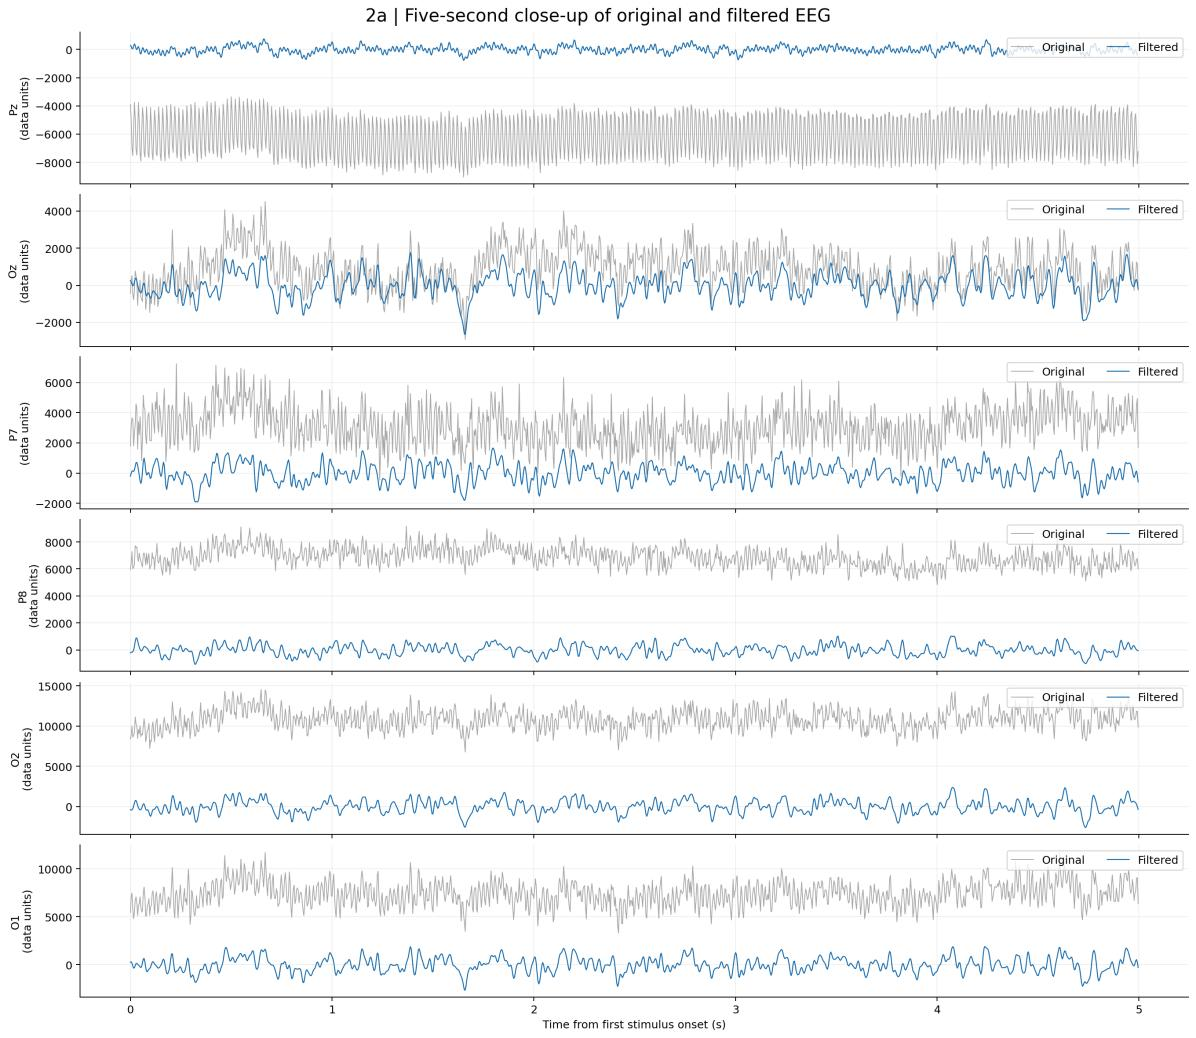
\includegraphics[width=0.9\textwidth]{fig06_ssvep_bandpass_filter_check.png}
\caption{The original signal and the output of the 1 to 40~Hz filter in the first five seconds of the first stimulus, for all six channels.}
\label{fig:ssvepfilter}
\end{figure}

\subsection*{(b) and (c) Windowing and spectrum estimation}
\begin{taskbox}
\textbf{(b)} Extract the 15 trials corresponding to the 15 stimuli, each with a 5-second window.\\
\textbf{(c)} For each trial, compute the frequency content of all six channels and plot them in one figure. You can use the function \texttt{pwelch}. Use an appropriate legend to indicate which channel each curve belongs to.
\end{taskbox}

\paragraph{(b) Separating the fifteen repetitions.} The start index of each stimulus was read from the variable \texttt{Event\_Samples}. Since MATLAB's index starts from one and Python's from zero, one unit was subtracted from each number. From the start of each stimulus, exactly five seconds, or 1250 samples, were taken. The final array has dimensions 15 repetitions $\times$ 6 channels $\times$ 1250 samples, and the completeness of all windows was checked.

\paragraph{(c) Computing the power spectral density.} The power spectral density of each channel in each repetition was computed with Welch's method. A Hann window of 625 samples, an overlap of 312 samples and an FFT length of 4096 were used. The basic frequency spacing corresponding to the segment length, $f_s/L$, is 0.4~Hz; the true resolving power also depends on the window shape. Zero-padding makes the display grid finer, with a spacing of about 0.061~Hz, but it does not increase the true resolution of the information. For each repetition, the six spectra are drawn in one figure with a legend of channel names; in addition to 15 separate figures, a collective view was also prepared.

The fifteen six-channel spectra are given separately in Appendix~A. The sample display of channel Oz in the figure below shows that the lengths of the windows are identical and that the time starts from the moment of the stimulus.

\begin{figure}[H]
\centering
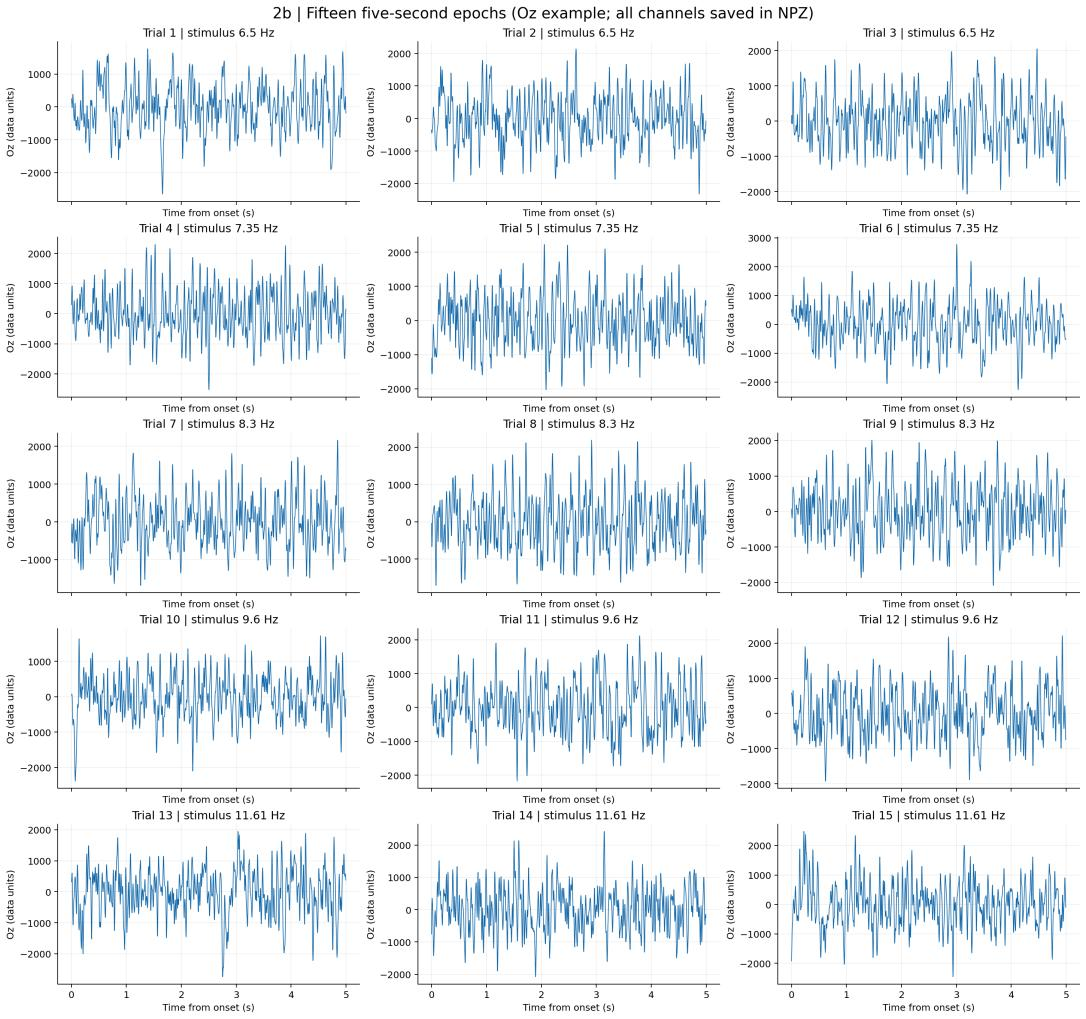
\includegraphics[width=0.9\textwidth]{fig07_ssvep_fifteen_windows_oz.png}
\caption{The fifteen five-second windows; channel Oz was chosen for display, and the spectral analysis was performed on all six channels.}
\label{fig:ssvepwin}
\end{figure}

\subsection*{(d) and (e) Differences between the channels and detection of the frequency}
\begin{taskbox}
\textbf{(d)} For a single trial, do all channels have the same frequency content? What is the reason for the differences in the frequency content of the channels?\\
\textbf{(e)} For each trial, can you determine the dominant frequency using the frequency content of the channels? To which frequencies do the spectral peaks correspond? Why does each of these peaks arise?
\end{taskbox}

\paragraph{(d) Comparison of the channels.} The spectra of the six channels are not identical in amplitude and shape. In this data, the mean power at the target frequency in the posterior channels Oz, O1 and O2 is higher than in Pz. The electrode location, the combination of sources and volume conduction, electrode noise and the background EEG can play a role in this difference; the present data do not determine the physiological cause of each difference conclusively.

\paragraph{(e) Fundamental frequency and harmonics.} To avoid mistaking slow background activity for the stimulation frequency, the simple search for the highest peak was explicitly performed in the range of 5 to 40~Hz. In 8 of the 15 repetitions, this peak is near the second harmonic of the stimulus. For the 6.5 and 7.35~Hz stimuli, the dominant peaks are seen at about 13 and 14.7~Hz, respectively. In the 8.3~Hz group, two repetitions have a dominant peak near 16.6~Hz and one repetition has a dominant peak near the fundamental frequency. In the 9.6 and 11.61~Hz groups, the dominant peak is mainly near the fundamental frequency. The highest peak of the spectrum is therefore not necessarily the stimulation frequency itself.

Peaks at multiples can arise from the non-sinusoidal shape of the response or from the nonlinearity of the visual pathway. Other peaks may also be related to the background EEG, alpha activity, artifacts or spectral leakage. Comparing the power at the five permitted fundamental frequencies gave the correct answer in all 15 repetitions.

\begin{table}[H]
\centering
\caption{The peak was searched for in the range of 5 to 40~Hz; the output of the PSD at the permitted fundamental frequencies and of CCA is identical in all 15 rows.}
\begin{tabular}{@{}cccc@{}}
\toprule
\textbf{Repetition} & \textbf{Stimulus (Hz)} & \textbf{Highest peak (Hz)} & \textbf{Estimate of both methods (Hz)}\\
\midrule
1  & 6.5   & 12.939 & 6.5\\
2  & 6.5   & 12.939 & 6.5\\
3  & 6.5   & 13.062 & 6.5\\
4  & 7.35  & 14.648 & 7.35\\
5  & 7.35  & 14.648 & 7.35\\
6  & 7.35  & 14.648 & 7.35\\
7  & 8.3   & 16.541 & 8.3\\
8  & 8.3   & 8.362  & 8.3\\
9  & 8.3   & 16.663 & 8.3\\
10 & 9.6   & 9.521  & 9.6\\
11 & 9.6   & 9.705  & 9.6\\
12 & 9.6   & 9.644  & 9.6\\
13 & 11.61 & 11.658 & 11.61\\
14 & 11.61 & 11.536 & 11.61\\
15 & 11.61 & 11.597 & 11.61\\
\bottomrule
\end{tabular}
\end{table}

\subsection*{(f) A complementary multichannel method}
\begin{taskbox}
Do you know another method for determining the dominant frequency in the SSVEP signal that gives better results than using the frequency content of the individual channels? By searching the internet and relevant papers, name other methods for processing SSVEP signals and determining the dominant frequency.
\end{taskbox}

Canonical correlation analysis (CCA) compares a linear combination of the EEG channels with a linear combination of sine and cosine references. For each candidate frequency, a reference of the fundamental frequency and of the second and third harmonics was built. The largest canonical correlation is the score of the candidate, and the largest score determines the predicted frequency. The references are built identically for all five candidates; the true label of a repetition is not used in selecting the answer, and only the set of the permitted frequencies of the system is assumed known. Lin et al.\ introduced this approach for SSVEP detection in 2006.
\begin{equation}
\rho(f)=\max\operatorname{corr}(Xw,\,Y_f v);\qquad
\hat f=\arg\max_f\rho(f)
\end{equation}

CCA can use the joint temporal and spatial information of several channels. The FBCCA method, introduced by Chen et al.\ in 2015, combines the information of the bands and harmonics with a filter bank. TRCA, introduced by Nakanishi et al.\ in 2018, uses labeled training repetitions to learn a spatial filter and an individual template. In this exercise, the complementary method that was run is ordinary CCA; FBCCA and TRCA are introduced only as a research answer.

CCA gave 15 correct answers in the same 15 repetitions. Since the PSD baseline at the permitted candidates also has 15 correct answers, a numerical superiority of CCA was not observed in this sample. In addition, this accuracy is descriptive, obtained from one person and 15 repetitions, and is not an estimate of performance on independent persons or data.

\begin{figure}[H]
\centering
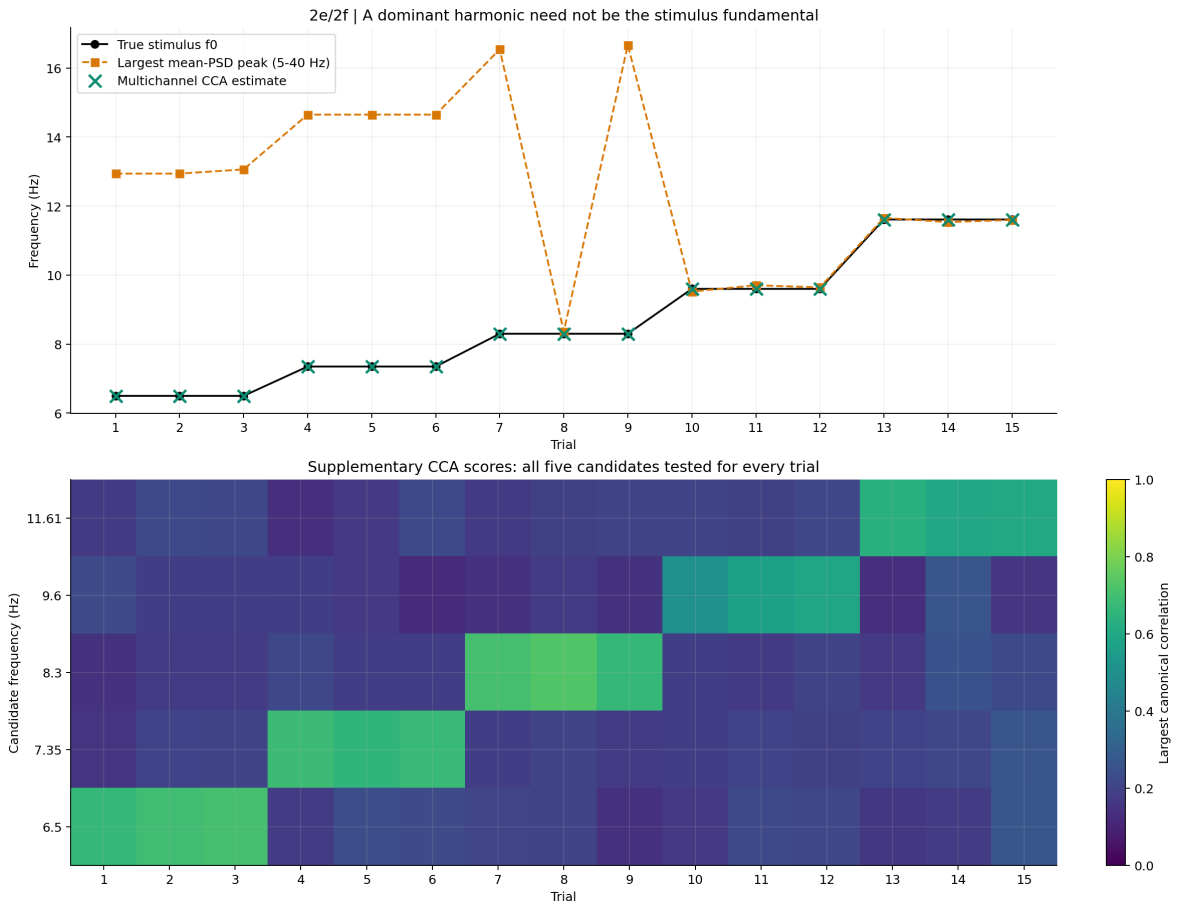
\includegraphics[width=0.8\textwidth]{fig08_ssvep_frequency_estimates.png}
\caption{Comparison of the true frequency, the highest peak and the CCA estimate; below, the score of all five candidates in each repetition is shown.}
\label{fig:ccaest}
\end{figure}
